\documentclass[border=3pt]{standalone}
% Shared TikZ styles for all paper figures.
%
% Colour is used to separate the two views (logical = blue, physical = ochre)
% and to mark the one emphasised relation (rose). Shape, line style and weight
% carry the same distinctions independently, so the figures still read when
% printed in black and white -- see the greyscale check in `make gray`.
\usepackage{tikz}
\usepackage{amsmath}
\usepackage[scaled=0.92]{helvet}
\renewcommand{\familydefault}{\sfdefault}
% Define \GRAYFIGS before % Shared TikZ styles for all paper figures.
%
% Colour is used to separate the two views (logical = blue, physical = ochre)
% and to mark the one emphasised relation (rose). Shape, line style and weight
% carry the same distinctions independently, so the figures still read when
% printed in black and white -- see the greyscale check in `make gray`.
\usepackage{tikz}
\usepackage{amsmath}
\usepackage[scaled=0.92]{helvet}
\renewcommand{\familydefault}{\sfdefault}
% Define \GRAYFIGS before % Shared TikZ styles for all paper figures.
%
% Colour is used to separate the two views (logical = blue, physical = ochre)
% and to mark the one emphasised relation (rose). Shape, line style and weight
% carry the same distinctions independently, so the figures still read when
% printed in black and white -- see the greyscale check in `make gray`.
\usepackage{tikz}
\usepackage{amsmath}
\usepackage[scaled=0.92]{helvet}
\renewcommand{\familydefault}{\sfdefault}
% Define \GRAYFIGS before \input{figstyle} to build the same figures in
% greyscale (xcolor converts every colour below), e.g.
%   pdflatex -jobname=fig1_gray "\def\GRAYFIGS{}\input{fig1_concept}"
\ifdefined\GRAYFIGS
  \usepackage[gray]{xcolor}
\else
  \usepackage{xcolor}
\fi
\usetikzlibrary{arrows.meta,positioning,fit,backgrounds,calc,shapes.geometric,
                shapes.misc,decorations.pathreplacing,patterns,matrix,shadows.blur}

% ------------------------------- palette -----------------------------------
\definecolor{ink}{HTML}{22333F}        % primary text
\definecolor{inkSoft}{HTML}{6B8299}    % secondary text, hairlines
\definecolor{astLine}{HTML}{2C7A9B}    % logical view
\definecolor{astFill}{HTML}{E7F2F7}
\definecolor{pdfLine}{HTML}{B0762F}    % physical view
\definecolor{pdfFill}{HTML}{FBF2E3}
\definecolor{hotLine}{HTML}{B03A55}    % the emphasised relation
\definecolor{hotFill}{HTML}{FBE9EC}
\definecolor{mutedLine}{HTML}{9FB3C8}  % furniture / unmatched
\definecolor{mutedFill}{HTML}{F1F5F8}

\tikzset{
  every node/.append style = {text=ink},
  >=Stealth,
  % --- logical structure (AST) -------------------------------------------
  astnode/.style   = {draw=astLine!70, fill=white, rounded corners=2.5pt,
                      line width=0.6pt, font=\scriptsize,
                      inner xsep=4pt, inner ysep=2.5pt, minimum height=4.6mm},
  astroot/.style   = {astnode, fill=astLine, draw=astLine, text=white},
  astsec/.style    = {astnode, fill=astFill},
  asttree/.style   = {draw=astLine!50, line width=0.6pt, rounded corners=2.5pt},
  % --- physical layout (page regions) ------------------------------------
  page/.style      = {draw=inkSoft!45, fill=white, line width=0.6pt,
                      rounded corners=2pt},
  lbox/.style      = {draw=pdfLine!55, fill=white, line width=0.6pt,
                      rounded corners=1.2pt},
  lboxhi/.style    = {draw=hotLine, fill=hotFill, line width=1.0pt,
                      rounded corners=1.2pt},
  furniture/.style = {draw=mutedLine, dash pattern=on 1.6pt off 1.4pt,
                      fill=mutedFill, line width=0.6pt, rounded corners=1.2pt},
  % --- relations ----------------------------------------------------------
  maplink/.style   = {draw=inkSoft, line width=0.6pt,
                      -{Stealth[length=1.7mm,width=1.3mm]}},
  maphot/.style    = {draw=hotLine, line width=1.1pt,
                      -{Stealth[length=2mm,width=1.6mm]}},
  flow/.style      = {draw=inkSoft, line width=0.7pt,
                      -{Stealth[length=2mm,width=1.6mm]}, rounded corners=2pt},
  % --- pipeline stages ----------------------------------------------------
  stage/.style     = {draw=inkSoft!55, fill=white, rounded corners=2.5pt,
                      font=\scriptsize, align=center, inner sep=3.5pt,
                      minimum height=7mm, text width=32mm},
  artefact/.style  = {draw=inkSoft!35, fill=mutedFill, rounded corners=2.5pt,
                      font=\scriptsize, align=center, inner sep=3.5pt,
                      minimum height=7mm, text width=32mm},
  % --- labels -------------------------------------------------------------
  grouplbl/.style  = {font=\scriptsize, text=inkSoft},
  caption/.style   = {font=\scriptsize, text=ink},
  tinylbl/.style   = {font=\tiny, text=inkSoft},
  softcard/.style  = {rounded corners=4pt, draw=none},
}

% Fake text lines inside a layout box.
% [colour] {x} {y top} {width} {line count}
\newcommand{\fakelines}[5][pdfLine!32]{%
  \foreach \fli in {1,...,#5}{%
    \draw[#1, line width=0.32pt] (#2,{#3-0.115*\fli}) -- ++({#4},0);}%
}
% Same, with a short final line (end of a paragraph)
\newcommand{\fakepara}[5][pdfLine!32]{%
  \foreach \fli in {1,...,#5}{%
    \draw[#1, line width=0.32pt] (#2,{#3-0.115*\fli}) -- ++({#4},0);}%
  \draw[#1, line width=0.32pt] (#2,{#3-0.115*(#5+1)}) -- ++({0.55*#4},0);%
}
 to build the same figures in
% greyscale (xcolor converts every colour below), e.g.
%   pdflatex -jobname=fig1_gray "\def\GRAYFIGS{}\documentclass[border=3pt]{standalone}
\input{figstyle}
\begin{document}
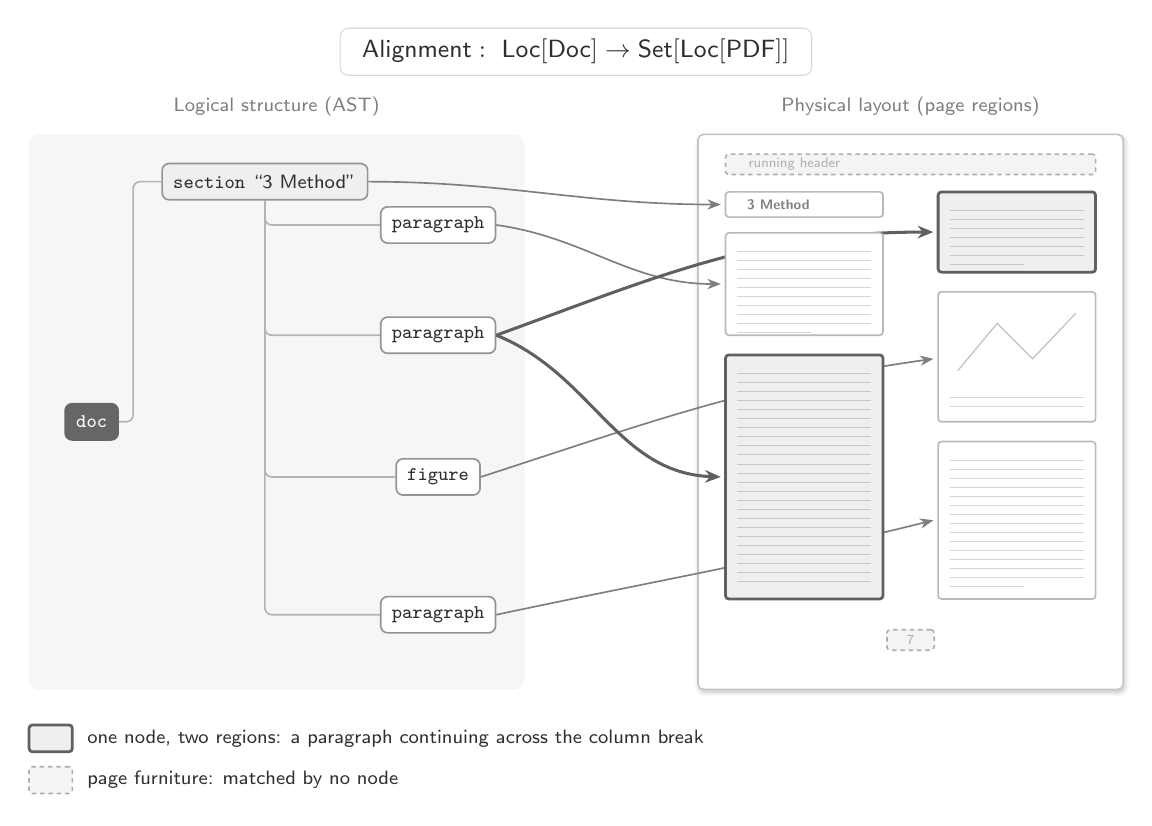
\begin{tikzpicture}

% ============================ title badge ==================================
\node[rounded corners=3pt, draw=inkSoft!30, fill=white, inner xsep=8pt,
      inner ysep=4pt, font=\small] at (6.95,8.00)
     {$\mathsf{Alignment}:\ \mathsf{Loc}[\mathsf{Doc}] \rightarrow
       \mathsf{Set}[\mathsf{Loc}[\mathsf{PDF}]]$};

\node[grouplbl] at (3.15,7.30) {Logical structure (AST)};
\node[grouplbl] at (11.20,7.30) {Physical layout (page regions)};

% ============================ the two cards ================================
\fill[softcard, fill=astFill!55] (0.00,-0.10) rectangle (6.30,6.95);
\node[page, fit={(8.50,-0.10) (13.90,6.95)}, inner sep=0pt,
      blur shadow={shadow blur steps=8, shadow xshift=0.5pt,
                   shadow yshift=-0.9pt, shadow opacity=25}] {};

% ======================= LEFT: logical structure (AST) =====================
\node[astroot] (doc)  at (0.80,3.30) {\texttt{doc}};
\node[astsec]  (sec1) at (3.00,6.35) {\texttt{section} ``3 Method''};
\node[astnode] (p1)   at (5.20,5.80) {\texttt{paragraph}};
\node[astnode] (p2)   at (5.20,4.40) {\texttt{paragraph}};
\node[astnode] (fg)   at (5.20,2.60) {\texttt{figure}};
\node[astnode] (p3)   at (5.20,0.85) {\texttt{paragraph}};

\draw[asttree] (doc.east) -- ++(0.18,0) |- (sec1.west);
\foreach \c in {p1,p2,fg,p3}{ \draw[asttree] (sec1.south) |- (\c.west); }

% ============================= THE MAPPING =================================
% (drawn before the regions, so the links pass behind them)
\draw[maplink] (sec1.east) to[out=0,in=180]   (8.79,6.06);
\draw[maplink] (p1.east)   to[out=-8,in=180]  (8.79,5.05);
\draw[maplink] (fg.east)   to[out=18,in=188]  (11.49,4.10);
\draw[maplink] (p3.east)   to[out=12,in=194]  (11.49,2.05);

% one node, two regions, split across the column break
\draw[maphot]  (p2.east) to[out=-22,in=178] (8.79,2.60);
\draw[maphot]  (p2.east) to[out=20,in=180]  (11.49,5.71);

% ======================= page regions (opaque, on top) =====================
\node[furniture, fit={(8.85,6.44) (13.55,6.70)}, inner sep=0pt] {};
\node[font=\tiny, text=mutedLine, anchor=west] at (9.02,6.57) {running header};
\node[furniture, fit={(10.90,0.40) (11.50,0.66)}, inner sep=0pt] {};
\node[font=\tiny, text=mutedLine] at (11.20,0.53) {7};

% --- left column ---
\node[lbox, fit={(8.85,5.90) (10.85,6.22)}, inner sep=0pt] {};
\node[font=\tiny, text=pdfLine, anchor=west] at (9.00,6.06) {\textbf{3 Method}};

\node[lbox, fit={(8.85,4.40) (10.85,5.70)}, inner sep=0pt] {};
\fakepara{9.00}{5.58}{1.70}{9}

\node[lboxhi, fit={(8.85,1.05) (10.85,4.15)}, inner sep=0pt] {};
\fakelines[hotLine!35]{9.00}{4.03}{1.70}{24}

% --- right column ---
\node[lboxhi, fit={(11.55,5.20) (13.55,6.22)}, inner sep=0pt] {};
\fakepara[hotLine!35]{11.70}{6.10}{1.70}{6}

\node[lbox, fit={(11.55,3.30) (13.55,4.95)}, inner sep=0pt] {};
\draw[pdfLine!45, line width=0.5pt, line join=round]
      (11.80,3.95) -- (12.30,4.55) -- (12.75,4.10) -- (13.30,4.68);
\fakelines{11.70}{3.72}{1.70}{2}

\node[lbox, fit={(11.55,1.05) (13.55,3.05)}, inner sep=0pt] {};
\fakepara{11.70}{2.93}{1.70}{14}

% ================================ legend ===================================
\node[lboxhi, minimum width=5.5mm, minimum height=3.4mm, inner sep=0pt]
      at (0.28,-0.72) {};
\node[caption, anchor=west] at (0.62,-0.72)
     {one node, two regions: a paragraph continuing across the column break};

\node[furniture, minimum width=5.5mm, minimum height=3.4mm, inner sep=0pt]
      at (0.28,-1.25) {};
\node[caption, anchor=west] at (0.62,-1.25)
     {page furniture: matched by no node};

\end{tikzpicture}
\end{document}
"
\ifdefined\GRAYFIGS
  \usepackage[gray]{xcolor}
\else
  \usepackage{xcolor}
\fi
\usetikzlibrary{arrows.meta,positioning,fit,backgrounds,calc,shapes.geometric,
                shapes.misc,decorations.pathreplacing,patterns,matrix,shadows.blur}

% ------------------------------- palette -----------------------------------
\definecolor{ink}{HTML}{22333F}        % primary text
\definecolor{inkSoft}{HTML}{6B8299}    % secondary text, hairlines
\definecolor{astLine}{HTML}{2C7A9B}    % logical view
\definecolor{astFill}{HTML}{E7F2F7}
\definecolor{pdfLine}{HTML}{B0762F}    % physical view
\definecolor{pdfFill}{HTML}{FBF2E3}
\definecolor{hotLine}{HTML}{B03A55}    % the emphasised relation
\definecolor{hotFill}{HTML}{FBE9EC}
\definecolor{mutedLine}{HTML}{9FB3C8}  % furniture / unmatched
\definecolor{mutedFill}{HTML}{F1F5F8}

\tikzset{
  every node/.append style = {text=ink},
  >=Stealth,
  % --- logical structure (AST) -------------------------------------------
  astnode/.style   = {draw=astLine!70, fill=white, rounded corners=2.5pt,
                      line width=0.6pt, font=\scriptsize,
                      inner xsep=4pt, inner ysep=2.5pt, minimum height=4.6mm},
  astroot/.style   = {astnode, fill=astLine, draw=astLine, text=white},
  astsec/.style    = {astnode, fill=astFill},
  asttree/.style   = {draw=astLine!50, line width=0.6pt, rounded corners=2.5pt},
  % --- physical layout (page regions) ------------------------------------
  page/.style      = {draw=inkSoft!45, fill=white, line width=0.6pt,
                      rounded corners=2pt},
  lbox/.style      = {draw=pdfLine!55, fill=white, line width=0.6pt,
                      rounded corners=1.2pt},
  lboxhi/.style    = {draw=hotLine, fill=hotFill, line width=1.0pt,
                      rounded corners=1.2pt},
  furniture/.style = {draw=mutedLine, dash pattern=on 1.6pt off 1.4pt,
                      fill=mutedFill, line width=0.6pt, rounded corners=1.2pt},
  % --- relations ----------------------------------------------------------
  maplink/.style   = {draw=inkSoft, line width=0.6pt,
                      -{Stealth[length=1.7mm,width=1.3mm]}},
  maphot/.style    = {draw=hotLine, line width=1.1pt,
                      -{Stealth[length=2mm,width=1.6mm]}},
  flow/.style      = {draw=inkSoft, line width=0.7pt,
                      -{Stealth[length=2mm,width=1.6mm]}, rounded corners=2pt},
  % --- pipeline stages ----------------------------------------------------
  stage/.style     = {draw=inkSoft!55, fill=white, rounded corners=2.5pt,
                      font=\scriptsize, align=center, inner sep=3.5pt,
                      minimum height=7mm, text width=32mm},
  artefact/.style  = {draw=inkSoft!35, fill=mutedFill, rounded corners=2.5pt,
                      font=\scriptsize, align=center, inner sep=3.5pt,
                      minimum height=7mm, text width=32mm},
  % --- labels -------------------------------------------------------------
  grouplbl/.style  = {font=\scriptsize, text=inkSoft},
  caption/.style   = {font=\scriptsize, text=ink},
  tinylbl/.style   = {font=\tiny, text=inkSoft},
  softcard/.style  = {rounded corners=4pt, draw=none},
}

% Fake text lines inside a layout box.
% [colour] {x} {y top} {width} {line count}
\newcommand{\fakelines}[5][pdfLine!32]{%
  \foreach \fli in {1,...,#5}{%
    \draw[#1, line width=0.32pt] (#2,{#3-0.115*\fli}) -- ++({#4},0);}%
}
% Same, with a short final line (end of a paragraph)
\newcommand{\fakepara}[5][pdfLine!32]{%
  \foreach \fli in {1,...,#5}{%
    \draw[#1, line width=0.32pt] (#2,{#3-0.115*\fli}) -- ++({#4},0);}%
  \draw[#1, line width=0.32pt] (#2,{#3-0.115*(#5+1)}) -- ++({0.55*#4},0);%
}
 to build the same figures in
% greyscale (xcolor converts every colour below), e.g.
%   pdflatex -jobname=fig1_gray "\def\GRAYFIGS{}\documentclass[border=3pt]{standalone}
% Shared TikZ styles for all paper figures.
%
% Colour is used to separate the two views (logical = blue, physical = ochre)
% and to mark the one emphasised relation (rose). Shape, line style and weight
% carry the same distinctions independently, so the figures still read when
% printed in black and white -- see the greyscale check in `make gray`.
\usepackage{tikz}
\usepackage{amsmath}
\usepackage[scaled=0.92]{helvet}
\renewcommand{\familydefault}{\sfdefault}
% Define \GRAYFIGS before \input{figstyle} to build the same figures in
% greyscale (xcolor converts every colour below), e.g.
%   pdflatex -jobname=fig1_gray "\def\GRAYFIGS{}\input{fig1_concept}"
\ifdefined\GRAYFIGS
  \usepackage[gray]{xcolor}
\else
  \usepackage{xcolor}
\fi
\usetikzlibrary{arrows.meta,positioning,fit,backgrounds,calc,shapes.geometric,
                shapes.misc,decorations.pathreplacing,patterns,matrix,shadows.blur}

% ------------------------------- palette -----------------------------------
\definecolor{ink}{HTML}{22333F}        % primary text
\definecolor{inkSoft}{HTML}{6B8299}    % secondary text, hairlines
\definecolor{astLine}{HTML}{2C7A9B}    % logical view
\definecolor{astFill}{HTML}{E7F2F7}
\definecolor{pdfLine}{HTML}{B0762F}    % physical view
\definecolor{pdfFill}{HTML}{FBF2E3}
\definecolor{hotLine}{HTML}{B03A55}    % the emphasised relation
\definecolor{hotFill}{HTML}{FBE9EC}
\definecolor{mutedLine}{HTML}{9FB3C8}  % furniture / unmatched
\definecolor{mutedFill}{HTML}{F1F5F8}

\tikzset{
  every node/.append style = {text=ink},
  >=Stealth,
  % --- logical structure (AST) -------------------------------------------
  astnode/.style   = {draw=astLine!70, fill=white, rounded corners=2.5pt,
                      line width=0.6pt, font=\scriptsize,
                      inner xsep=4pt, inner ysep=2.5pt, minimum height=4.6mm},
  astroot/.style   = {astnode, fill=astLine, draw=astLine, text=white},
  astsec/.style    = {astnode, fill=astFill},
  asttree/.style   = {draw=astLine!50, line width=0.6pt, rounded corners=2.5pt},
  % --- physical layout (page regions) ------------------------------------
  page/.style      = {draw=inkSoft!45, fill=white, line width=0.6pt,
                      rounded corners=2pt},
  lbox/.style      = {draw=pdfLine!55, fill=white, line width=0.6pt,
                      rounded corners=1.2pt},
  lboxhi/.style    = {draw=hotLine, fill=hotFill, line width=1.0pt,
                      rounded corners=1.2pt},
  furniture/.style = {draw=mutedLine, dash pattern=on 1.6pt off 1.4pt,
                      fill=mutedFill, line width=0.6pt, rounded corners=1.2pt},
  % --- relations ----------------------------------------------------------
  maplink/.style   = {draw=inkSoft, line width=0.6pt,
                      -{Stealth[length=1.7mm,width=1.3mm]}},
  maphot/.style    = {draw=hotLine, line width=1.1pt,
                      -{Stealth[length=2mm,width=1.6mm]}},
  flow/.style      = {draw=inkSoft, line width=0.7pt,
                      -{Stealth[length=2mm,width=1.6mm]}, rounded corners=2pt},
  % --- pipeline stages ----------------------------------------------------
  stage/.style     = {draw=inkSoft!55, fill=white, rounded corners=2.5pt,
                      font=\scriptsize, align=center, inner sep=3.5pt,
                      minimum height=7mm, text width=32mm},
  artefact/.style  = {draw=inkSoft!35, fill=mutedFill, rounded corners=2.5pt,
                      font=\scriptsize, align=center, inner sep=3.5pt,
                      minimum height=7mm, text width=32mm},
  % --- labels -------------------------------------------------------------
  grouplbl/.style  = {font=\scriptsize, text=inkSoft},
  caption/.style   = {font=\scriptsize, text=ink},
  tinylbl/.style   = {font=\tiny, text=inkSoft},
  softcard/.style  = {rounded corners=4pt, draw=none},
}

% Fake text lines inside a layout box.
% [colour] {x} {y top} {width} {line count}
\newcommand{\fakelines}[5][pdfLine!32]{%
  \foreach \fli in {1,...,#5}{%
    \draw[#1, line width=0.32pt] (#2,{#3-0.115*\fli}) -- ++({#4},0);}%
}
% Same, with a short final line (end of a paragraph)
\newcommand{\fakepara}[5][pdfLine!32]{%
  \foreach \fli in {1,...,#5}{%
    \draw[#1, line width=0.32pt] (#2,{#3-0.115*\fli}) -- ++({#4},0);}%
  \draw[#1, line width=0.32pt] (#2,{#3-0.115*(#5+1)}) -- ++({0.55*#4},0);%
}

\begin{document}
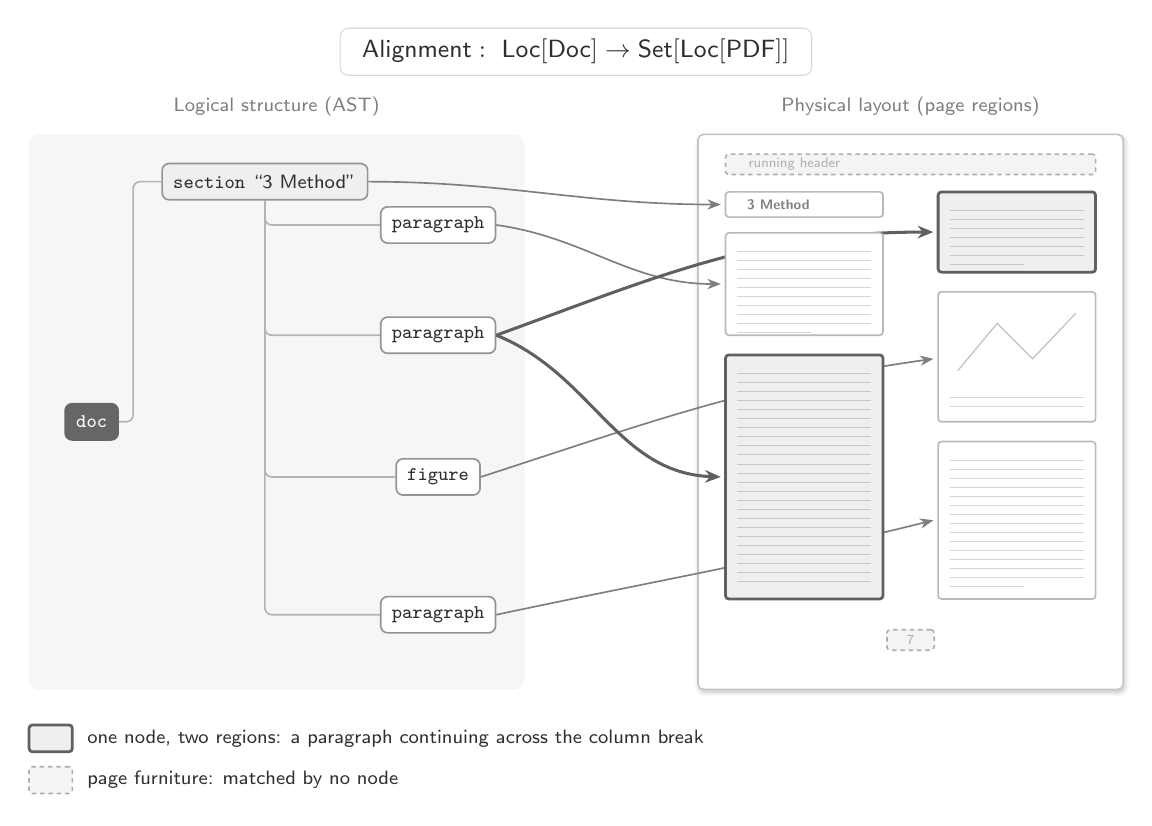
\begin{tikzpicture}

% ============================ title badge ==================================
\node[rounded corners=3pt, draw=inkSoft!30, fill=white, inner xsep=8pt,
      inner ysep=4pt, font=\small] at (6.95,8.00)
     {$\mathsf{Alignment}:\ \mathsf{Loc}[\mathsf{Doc}] \rightarrow
       \mathsf{Set}[\mathsf{Loc}[\mathsf{PDF}]]$};

\node[grouplbl] at (3.15,7.30) {Logical structure (AST)};
\node[grouplbl] at (11.20,7.30) {Physical layout (page regions)};

% ============================ the two cards ================================
\fill[softcard, fill=astFill!55] (0.00,-0.10) rectangle (6.30,6.95);
\node[page, fit={(8.50,-0.10) (13.90,6.95)}, inner sep=0pt,
      blur shadow={shadow blur steps=8, shadow xshift=0.5pt,
                   shadow yshift=-0.9pt, shadow opacity=25}] {};

% ======================= LEFT: logical structure (AST) =====================
\node[astroot] (doc)  at (0.80,3.30) {\texttt{doc}};
\node[astsec]  (sec1) at (3.00,6.35) {\texttt{section} ``3 Method''};
\node[astnode] (p1)   at (5.20,5.80) {\texttt{paragraph}};
\node[astnode] (p2)   at (5.20,4.40) {\texttt{paragraph}};
\node[astnode] (fg)   at (5.20,2.60) {\texttt{figure}};
\node[astnode] (p3)   at (5.20,0.85) {\texttt{paragraph}};

\draw[asttree] (doc.east) -- ++(0.18,0) |- (sec1.west);
\foreach \c in {p1,p2,fg,p3}{ \draw[asttree] (sec1.south) |- (\c.west); }

% ============================= THE MAPPING =================================
% (drawn before the regions, so the links pass behind them)
\draw[maplink] (sec1.east) to[out=0,in=180]   (8.79,6.06);
\draw[maplink] (p1.east)   to[out=-8,in=180]  (8.79,5.05);
\draw[maplink] (fg.east)   to[out=18,in=188]  (11.49,4.10);
\draw[maplink] (p3.east)   to[out=12,in=194]  (11.49,2.05);

% one node, two regions, split across the column break
\draw[maphot]  (p2.east) to[out=-22,in=178] (8.79,2.60);
\draw[maphot]  (p2.east) to[out=20,in=180]  (11.49,5.71);

% ======================= page regions (opaque, on top) =====================
\node[furniture, fit={(8.85,6.44) (13.55,6.70)}, inner sep=0pt] {};
\node[font=\tiny, text=mutedLine, anchor=west] at (9.02,6.57) {running header};
\node[furniture, fit={(10.90,0.40) (11.50,0.66)}, inner sep=0pt] {};
\node[font=\tiny, text=mutedLine] at (11.20,0.53) {7};

% --- left column ---
\node[lbox, fit={(8.85,5.90) (10.85,6.22)}, inner sep=0pt] {};
\node[font=\tiny, text=pdfLine, anchor=west] at (9.00,6.06) {\textbf{3 Method}};

\node[lbox, fit={(8.85,4.40) (10.85,5.70)}, inner sep=0pt] {};
\fakepara{9.00}{5.58}{1.70}{9}

\node[lboxhi, fit={(8.85,1.05) (10.85,4.15)}, inner sep=0pt] {};
\fakelines[hotLine!35]{9.00}{4.03}{1.70}{24}

% --- right column ---
\node[lboxhi, fit={(11.55,5.20) (13.55,6.22)}, inner sep=0pt] {};
\fakepara[hotLine!35]{11.70}{6.10}{1.70}{6}

\node[lbox, fit={(11.55,3.30) (13.55,4.95)}, inner sep=0pt] {};
\draw[pdfLine!45, line width=0.5pt, line join=round]
      (11.80,3.95) -- (12.30,4.55) -- (12.75,4.10) -- (13.30,4.68);
\fakelines{11.70}{3.72}{1.70}{2}

\node[lbox, fit={(11.55,1.05) (13.55,3.05)}, inner sep=0pt] {};
\fakepara{11.70}{2.93}{1.70}{14}

% ================================ legend ===================================
\node[lboxhi, minimum width=5.5mm, minimum height=3.4mm, inner sep=0pt]
      at (0.28,-0.72) {};
\node[caption, anchor=west] at (0.62,-0.72)
     {one node, two regions: a paragraph continuing across the column break};

\node[furniture, minimum width=5.5mm, minimum height=3.4mm, inner sep=0pt]
      at (0.28,-1.25) {};
\node[caption, anchor=west] at (0.62,-1.25)
     {page furniture: matched by no node};

\end{tikzpicture}
\end{document}
"
\ifdefined\GRAYFIGS
  \usepackage[gray]{xcolor}
\else
  \usepackage{xcolor}
\fi
\usetikzlibrary{arrows.meta,positioning,fit,backgrounds,calc,shapes.geometric,
                shapes.misc,decorations.pathreplacing,patterns,matrix,shadows.blur}

% ------------------------------- palette -----------------------------------
\definecolor{ink}{HTML}{22333F}        % primary text
\definecolor{inkSoft}{HTML}{6B8299}    % secondary text, hairlines
\definecolor{astLine}{HTML}{2C7A9B}    % logical view
\definecolor{astFill}{HTML}{E7F2F7}
\definecolor{pdfLine}{HTML}{B0762F}    % physical view
\definecolor{pdfFill}{HTML}{FBF2E3}
\definecolor{hotLine}{HTML}{B03A55}    % the emphasised relation
\definecolor{hotFill}{HTML}{FBE9EC}
\definecolor{mutedLine}{HTML}{9FB3C8}  % furniture / unmatched
\definecolor{mutedFill}{HTML}{F1F5F8}

\tikzset{
  every node/.append style = {text=ink},
  >=Stealth,
  % --- logical structure (AST) -------------------------------------------
  astnode/.style   = {draw=astLine!70, fill=white, rounded corners=2.5pt,
                      line width=0.6pt, font=\scriptsize,
                      inner xsep=4pt, inner ysep=2.5pt, minimum height=4.6mm},
  astroot/.style   = {astnode, fill=astLine, draw=astLine, text=white},
  astsec/.style    = {astnode, fill=astFill},
  asttree/.style   = {draw=astLine!50, line width=0.6pt, rounded corners=2.5pt},
  % --- physical layout (page regions) ------------------------------------
  page/.style      = {draw=inkSoft!45, fill=white, line width=0.6pt,
                      rounded corners=2pt},
  lbox/.style      = {draw=pdfLine!55, fill=white, line width=0.6pt,
                      rounded corners=1.2pt},
  lboxhi/.style    = {draw=hotLine, fill=hotFill, line width=1.0pt,
                      rounded corners=1.2pt},
  furniture/.style = {draw=mutedLine, dash pattern=on 1.6pt off 1.4pt,
                      fill=mutedFill, line width=0.6pt, rounded corners=1.2pt},
  % --- relations ----------------------------------------------------------
  maplink/.style   = {draw=inkSoft, line width=0.6pt,
                      -{Stealth[length=1.7mm,width=1.3mm]}},
  maphot/.style    = {draw=hotLine, line width=1.1pt,
                      -{Stealth[length=2mm,width=1.6mm]}},
  flow/.style      = {draw=inkSoft, line width=0.7pt,
                      -{Stealth[length=2mm,width=1.6mm]}, rounded corners=2pt},
  % --- pipeline stages ----------------------------------------------------
  stage/.style     = {draw=inkSoft!55, fill=white, rounded corners=2.5pt,
                      font=\scriptsize, align=center, inner sep=3.5pt,
                      minimum height=7mm, text width=32mm},
  artefact/.style  = {draw=inkSoft!35, fill=mutedFill, rounded corners=2.5pt,
                      font=\scriptsize, align=center, inner sep=3.5pt,
                      minimum height=7mm, text width=32mm},
  % --- labels -------------------------------------------------------------
  grouplbl/.style  = {font=\scriptsize, text=inkSoft},
  caption/.style   = {font=\scriptsize, text=ink},
  tinylbl/.style   = {font=\tiny, text=inkSoft},
  softcard/.style  = {rounded corners=4pt, draw=none},
}

% Fake text lines inside a layout box.
% [colour] {x} {y top} {width} {line count}
\newcommand{\fakelines}[5][pdfLine!32]{%
  \foreach \fli in {1,...,#5}{%
    \draw[#1, line width=0.32pt] (#2,{#3-0.115*\fli}) -- ++({#4},0);}%
}
% Same, with a short final line (end of a paragraph)
\newcommand{\fakepara}[5][pdfLine!32]{%
  \foreach \fli in {1,...,#5}{%
    \draw[#1, line width=0.32pt] (#2,{#3-0.115*\fli}) -- ++({#4},0);}%
  \draw[#1, line width=0.32pt] (#2,{#3-0.115*(#5+1)}) -- ++({0.55*#4},0);%
}

\begin{document}
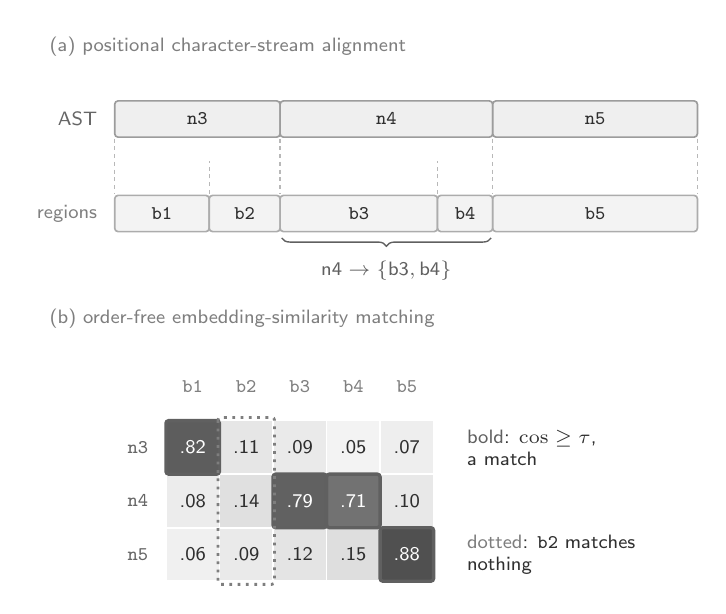
\begin{tikzpicture}[
  atape/.style = {draw=astLine!65, fill=astFill, line width=0.6pt, rounded corners=1.2pt},
  ptape/.style = {draw=pdfLine!65, fill=pdfFill, line width=0.6pt, rounded corners=1.2pt},
  tick/.style  = {draw=inkSoft!55, line width=0.45pt, dash pattern=on 1.4pt off 1.4pt},
  lbl/.style   = {font=\scriptsize},
  panel/.style = {font=\scriptsize, text=inkSoft},
]

% ==================== (a) positional stream aligner ========================
\node[panel, anchor=west] at (0.00,3.90) {(a) positional character-stream alignment};

\node[lbl, text=astLine, anchor=east] at (0.85,2.98) {AST};
\node[lbl, text=pdfLine, anchor=east] at (0.85,1.78) {regions};

% AST stream: three node spans
\foreach \x/\w/\lbl in {0.95/2.10/\texttt{n3}, 3.05/2.70/\texttt{n4}, 5.75/2.60/\texttt{n5}}{
  \draw[atape] (\x,2.75) rectangle ++(\w,0.46);
  \node[lbl] at ({\x+\w/2},2.98) {\lbl};}

% PDF stream: five box spans, in recovered reading order
\foreach \x/\w/\lbl in {0.95/1.20/\texttt{b1}, 2.15/0.90/\texttt{b2}, 3.05/2.00/\texttt{b3},
                        5.05/0.70/\texttt{b4}, 5.75/2.60/\texttt{b5}}{
  \draw[ptape] (\x,1.55) rectangle ++(\w,0.46);
  \node[lbl] at ({\x+\w/2},1.78) {\lbl};}

% character-position correspondence
\foreach \x in {0.95,3.05,5.75,8.35}{ \draw[tick] (\x,2.73) -- (\x,2.03); }
\foreach \x in {2.15,5.05}{ \draw[tick] (\x,2.03) -- (\x,2.45); }

\draw[decorate, decoration={brace, amplitude=3pt, mirror}, draw=hotLine,
      line width=0.5pt] (3.07,1.47) -- (5.73,1.47);
\node[lbl, text=hotLine, anchor=north] at (4.40,1.30)
      {$\mathsf{n4} \rightarrow \{\mathsf{b3},\mathsf{b4}\}$};

% ==================== (b) order-free similarity aligner ====================
\node[panel, anchor=west] at (0.00,0.45) {(b) order-free embedding-similarity matching};

% column headers
\foreach \c/\lbl in {1/\texttt{b1}, 2/\texttt{b2}, 3/\texttt{b3}, 4/\texttt{b4}, 5/\texttt{b5}}{
  \node[lbl, text=pdfLine] at ({1.60+(\c-1)*0.68+0.34},-0.42) {\lbl};}
% row headers
\foreach \r/\lbl in {1/\texttt{n3}, 2/\texttt{n4}, 3/\texttt{n5}}{
  \node[lbl, text=astLine, anchor=east] at (1.50,{-0.85-(\r-1)*0.68-0.34}) {\lbl};}

% similarity cells: shade = cosine
\foreach \r/\c/\s/\tc/\v in {%
  1/1/78/white/.82, 1/2/12/ink/.11, 1/3/10/ink/.09, 1/4/6/ink/.05, 1/5/8/ink/.07,
  2/1/9/ink/.08,  2/2/15/ink/.14, 2/3/76/white/.79, 2/4/68/white/.71, 2/5/11/ink/.10,
  3/1/7/ink/.06,  3/2/10/ink/.09, 3/3/13/ink/.12, 3/4/16/ink/.15, 3/5/84/white/.88}{
  \fill[ink!\s] ({1.60+(\c-1)*0.68},{-0.85-(\r-1)*0.68}) rectangle ++(0.68,-0.68);
  \draw[white, line width=0.6pt] ({1.60+(\c-1)*0.68},{-0.85-(\r-1)*0.68})
        rectangle ++(0.68,-0.68);
  \node[lbl, text=\tc] at ({1.60+(\c-1)*0.68+0.34},{-0.85-(\r-1)*0.68-0.34}) {\v};}

% cells above threshold
\foreach \r/\c in {1/1, 2/3, 2/4, 3/5}{
  \draw[hotLine, line width=1.2pt, rounded corners=1pt]
        ({1.60+(\c-1)*0.68},{-0.85-(\r-1)*0.68}) rectangle ++(0.68,-0.68);}

% b2 scores below the threshold against every node
\draw[dotted, draw=inkSoft, line width=1.0pt, rounded corners=1pt]
      (2.26,-0.81) rectangle (2.98,-2.93);

\node[lbl, anchor=west, align=left] at (5.30,-1.19)
     {\textcolor{hotLine}{bold}: $\cos \geq \tau$,\\ a match};
\node[lbl, anchor=west, align=left] at (5.30,-2.55)
     {\textcolor{inkSoft}{dotted}: \texttt{b2} matches\\ nothing};

\end{tikzpicture}
\end{document}
